\section{Auswertung}
\label{sec:Auswertung}
Die Messunsicherheiten des folgenden Kapitels wurden mit \textit{Python} unter Verwendung des Paketes \textit{scipy} \cite{scipy} bestimmt. Sie folgen aus der gaußschen
Fehlerfortpflanzung
\begin{equation}
  \label{eqn:Gauss}
  \Delta F = \sqrt{\sum_i\left(\frac{\symup{d}F}{\symup{d}y_i}\Delta y_i \right)^2}.
\end{equation} 

\subsection{Bestimmung der Winkelrichtgröße und des Eigenträgheitsmoments der Drehachse}
\label{subsec:A_Apparatenkonstanten}
Bevor mit dem eigentlichen Versuch begonnnen werden kann, müssen die Winkelrichtgröße $D$ der Feder und das Eigenträgheitsmoments $I_D$ der Drehachse ermittelt werden. 
Erstere kann mithilfe der Messwerte aus \autoref{tab:Winkelricht} durch \autoref{eqn:Winkelrichtgröße} bestimmt werden. Neben den Messwerten finden sich die jeweiligen 
Werte der Winkelrichtgröße in der genannten Tabelle.
\begin{table}
  \centering
  \caption{Messdaten zur Bestimmung der Winkelrichtgröße zum festen Abstand $a = \qty{20}{\centi\metre}$}
  \label{tab:Winkelricht}
  \begin{tabular}{S[table-format = 3.0] S[table-format = 1.3] S}
    \toprule
    {$\phi \mathbin{/} °$} & {$F \mathbin{/} \unit{\newton}$} & {$D \mathbin{/} \unit{\newton\metre\per\radian}$} \\
    \midrule
     20 & 0.025 & 0.029 \\
     30 & 0.045 & 0.034 \\
     40 & 0.067 & 0.038 \\
     50 & 0.1   & 0.046 \\
     60 & 0.124 & 0.047 \\
     70 & 0.145 & 0.047 \\
     80 & 0.17  & 0.049 \\
     90 & 0.25  & 0.064 \\
    100 & 0.27  & 0.062 \\
    110 & 0.3   & 0.063 \\
    \bottomrule
  \end{tabular}
\end{table}
Durch Mittelung der experimentellen Werte für die Winkelrichtgröße ergibt sich der Mittelwert $D = \qty{0.048 +- 0.012}{\newton\metre\per\radian}$.

Zur Bestimmung des Eigendrehmoments der Drehachse wird \autoref{eqn:Schwingungsdauer} betrachtet. Für das Quadrat der Schwingungsdauer $T$ ergibt sich
durch einsetzen des Gesamtträgheitsmoments $I = I_D + I_\text{Zylinder}$ unter Verwendung des Satzes von Steiner \eqref{eqn:Steiner}
\begin{equation}
  \label{eqn:I_D}
  T^2 = \frac{4\pi^2}{D}\left(I_D + 2I_\text{Z,h} + 2 m a^2) \right)
\end{equation}
mit der Masse $m = \qty{261.2}{\gram}$, dem Trägheitsmoment $I_\text{Z,h}$ eines zylinderförmigen Gewichtes und dem Abstand $a$ der Zylinder zur Drehachse. $I_\text{Z,h}$
berechnet sich dabei nach der Gleichung für einen horizontalen Zylinder aus \autoref{fig:Trägheitsmomente}.
Dies stellt eine Geradengleichung der Form $f(x) = mx^2 +b$ mit $f(x) = T^2(a^2)$ dar. In \autoref{fig:plot} sind die 
Quadrate der Messwerte für die Schwingungsdauer $T$ zum Abstand $a$ zur Drehachse aufgeführt. 
\begin{figure}
  \centering
  \includegraphics[width=0.8\textwidth]{plot.pdf}
  \caption{Graph der Quadrate der Messwerte und Ausgleichsgerade der linearen Regression. \cite{matplotlib}}
  \label{fig:plot}
\end{figure}
Eine lineare Regression mittels \textit{scipy} \cite{scipy} ergibt die Geradenparameter $m = \qty{732 +- 5}{\second\squared\per\metre\squared}$ und 
$b = \qty{5.62 +- 0.27}{\second\squared}$. Ein Koeffizientenvergleich von \autoref{eqn:I_D} und der Geradengleichung ergibt 
\begin{equation*}
  b = \frac{4\pi^2}{D}(I_D + 2I_\text{Z,h}),
\end{equation*}
woraus sich das Eigenträgheitsmoment $I_D$ bestimmen lässt. Mit dem Durchmesser $d = \qty{4.5}{\centi\metre}$ und der Höhe $h = \qty{2}{\centi\metre}$ der zylinderförmigen
Gewichte folgt $I_D = \qty{6.2 +- 1.6}{\gram\square\metre}$. Dieser Wert liegt eine Größenordnung über den im Folgenden zu bestimmenden Trägheitsmomenten, was nicht der 
Wahrheit entsprechen kann, da das Trägheitsmoment der Drehachse selbst sehr viel kleiner ist. Näheres hierzu findet sich in \autoref{sec:Diskussion}. Der wahre Wert von
$I_D$ wird für weitere Rechnungen als vernachlässigbar gering angenommen.
\subsection{Bestimmung des Trägheitsmomentes eines Zylinders}
\label{subsec:A_zylinder}
Der untersuchte Zylinder hatte eine Höhe von $h = \qty{10.09}{\centi\metre}$ und einen Durchmesser $d = \qty{9.83}{\centi\metre}$. Die Masse des Zylinder beträgt $m = \qty{367.7}{\gram}$.
Die Periodendauer wurde zehn mal gemessen mit jeweils fünffacher Periodendauer. Diese können \autoref{tab:einfacheKörper} entnommen werden. Zur Berechnung des Trägheitsmomentes werden die Einzelmessungen zunächst über 
fünf Perioden gemittelt und danach wird ein Mittelwert aus den zehn Werten genommen.
\begin{table}
    \centering
    \caption{Messung der Periodendauern von einfach Körpern. $T_z$ beschreibt die Periodendauer des Zylinders und $T_k$ die der Kugel.} 
    \label{tab:einfacheKörper}
    \begin{tabular}{c c}
        \toprule
        $\unit{{5}T_{z}\per\second}$ & $\unit{{5}T_k\per\second}$ \\
        \midrule
        3.81 & 9.29 \\
        3.76 & 9.20 \\
        3.77 & 9.43 \\
        3.78 & 9.37 \\
        3.74 & 9.24 \\
        3.85 & 9.40 \\
        3.82 & 9.32 \\
        3.84 & 9.21 \\
        3.86 & 9.28 \\
        3.77 & 9.30 \\
        \bottomrule 
    \end{tabular}
\end{table}
Die mittlere Periodendauer des Zylinders beträgt somit $\overline{T}_z = \qty{0.760+-0.008}{\second}$.
Mittels \autoref{eqn:I_K} kann das experimentelle Trägheitsmoment des Zylinders $I_{z,\text{exp}}$ berechnet werden. Durch einsetzen der Werte ergibt sich $I_{z,\text{exp}} = \qty{0.70+-0.18}{\gram\metre\squared}$.
Der Theoriewert $I_{z,\text{theo}}$ des Trägheitsmomentes eines Zylinders lässt sich nach der Formel für $I_z$ berechnen, welche \autoref{fig:Trägheitsmomente} entnommen werden kann.
Durch Einsetzen der Abmessungen des Zylinders kann $I_{z,\text{theo}} = \qty{0.444}{\gram\metre\squared}$ berechnet werden.
\subsection{Bestimmung des Trägheitsmomentes einer Kugel}
\label{subsec:A_kugel}
Die untersuchte Kugel hat einen Durchmesser von $d_k = \qty{14.72}{\centi\metre}$ und eine Masse von $m_k = \qty{1170.3}{\gram}$. Die Messwerte zur Periodendauer der Kugel
können \autoref{tab:einfacheKörper} entnommen werden. Wie schon in \autoref{subsec:A_zylinder} wird auch hier ein Mittelwert für die Berechnung vom Trägheitsmoment
verwendet. Die mittlere Periodendauer der Kugel liegt bei $\overline{T}_k = \qty{1.861+-0.016}{\second}$. Das experimentelle Trägheitsmoment $I_{k,\text{exp}}$ der Kugel 
lässt sich gemäß \autoref{eqn:I_K} berechnen. Dadurch ergibt sich $I_{k,\text{exp}} = \qty{4.2+-1.1}{\gram\metre\squared}$. Den Theoriewert zum Trägheitsmoment einer Kugel
kann man mit der Formel $I_{k,\text{theo}} = \frac{2}{5}m_k\left(\sfrac{d_k}{2}\right)^2$ berechnet werden, welche \autoref{fig:Trägheitsmomente} zu entnehmen ist.
Mit den gemessenen Größen ergibt $I_{k,\text{theo}} = \qty{2.53}{\gram\metre\squared}$. 
\subsection{Bestimmung des Trägheitsmomentes einer Holzpuppe}
\label{subsec:A_holzpuppe}
Das Trägheitsmoment einer Holzpuppe wird im folgendem für zwei unterschiedliche Stellungen der Puppe berechnet. Zuvor werden noch die Maaße der Puppe ausgewertet.
\begin{table}
  \centering
  \caption{Messdaten zur Bestimmung der Körpermodellierung. $d_k$ beschreibt den Durchmesser des Kopfes. Weiter beschreibt der Index a den Arm, r den Rumpf und b das Bein der Puppe.} 
  \label{tab:holzpuppe}
  \begin{tabular}{S S S S}
      \toprule
      $\unit{d_k\per\centi\metre}$ & $\unit{d_a\per\centi\metre}$ & $\unit{d_r\per\centi\metre}$ &  $\unit{d_b\per\centi\metre}$ \\
      \midrule
      2.61 & 1.30 & 3.86 & 1.92 \\
      2.86 & 1.38 & 3.76 & 1.91 \\
      2.90 & 1.40 & 3.55 & 1.80 \\
      2.83 & 1.46 & 3.00 & 1.60 \\
      2.66 & 1.20 & 3.52 & 1.56 \\
      2.21 & 1.37 & 3.73 & 1.60 \\
           & 1.47 & 4.00 & 1.70 \\
           & 1.23 & 4.22 & 1.62 \\
           & 1.12 &      & 1.40 \\
           & 1.27 &      & 1.30 \\
      \bottomrule 
  \end{tabular}
\end{table}
Aus diesen Durchmessern wird der Mittelwert gebildet, damit die einzelnen Körperteile als Zylinder genähert werden können.
Damit ergeben sich die Abmessungen vom Kopf mit der Länge $l_k = \qty{4.14}{\centi\metre}$, dem Radius $r_k = \qty{0.0134+-0.0013}{\centi\metre}$ und der Masse $m_k = \qty{0.018+-0.004}{\kilo\gram}$,
Die Arme mit $l_a = \qty{12.91}{\centi\metre}$, dem Radius $r_k = \qty{0.0066+-0.0006}{\centi\metre}$ und der Masse $m_k = \qty{0.0136+-0.0025}{\kilo\gram}$,
der Rumpf mit $l_r = \qty{9.84}{\centi\metre}$, dem Radius $r_k = \qty{0.0185+-0.0018}{\centi\metre}$ und der Masse $m_k = \qty{0.082+-0.010}{\kilo\gram}$ und das Bein mit
$l_b = \qty{12.42}{\centi\metre}$, dem Radius $r_k = \qty{0.0082+-0.0010}{\centi\metre}$ und der Masse $m_k = \qty{0.020+-0.004}{\kilo\gram}$. 
Die Massen wurden bestimmt indem zunächst die Volumina der einzelnen Körperteile berechnet wurden. Da alle Körperteile als Zylinder genähert wurden können dieser Volumina mit $V = \pi r^2h$ berechnet werden.
Daraus kann dann das Gessamtvolumen berechnet werden. Die einzelnen Massen wurden dann bestimmt indem der prozentuale Anteil des Volumens mit der Gesamtmasse multipliziert wurde.

\begin{figure}
  \centering
  \caption{Abbildung zur experimentellen Bestimmung der Trägheitsmomente komplexer Körper:In dieser Abbildung ist eine Stellung der verwendete Holzpuppe auf der Drill-Achse zu sehen.}
  \label{fig:D_subfig}
  \begin{subfigure}{0.48\textwidth}
      \centering
      \caption{Stellung 1}
      \label{fig:D_Holzpuppe1}
      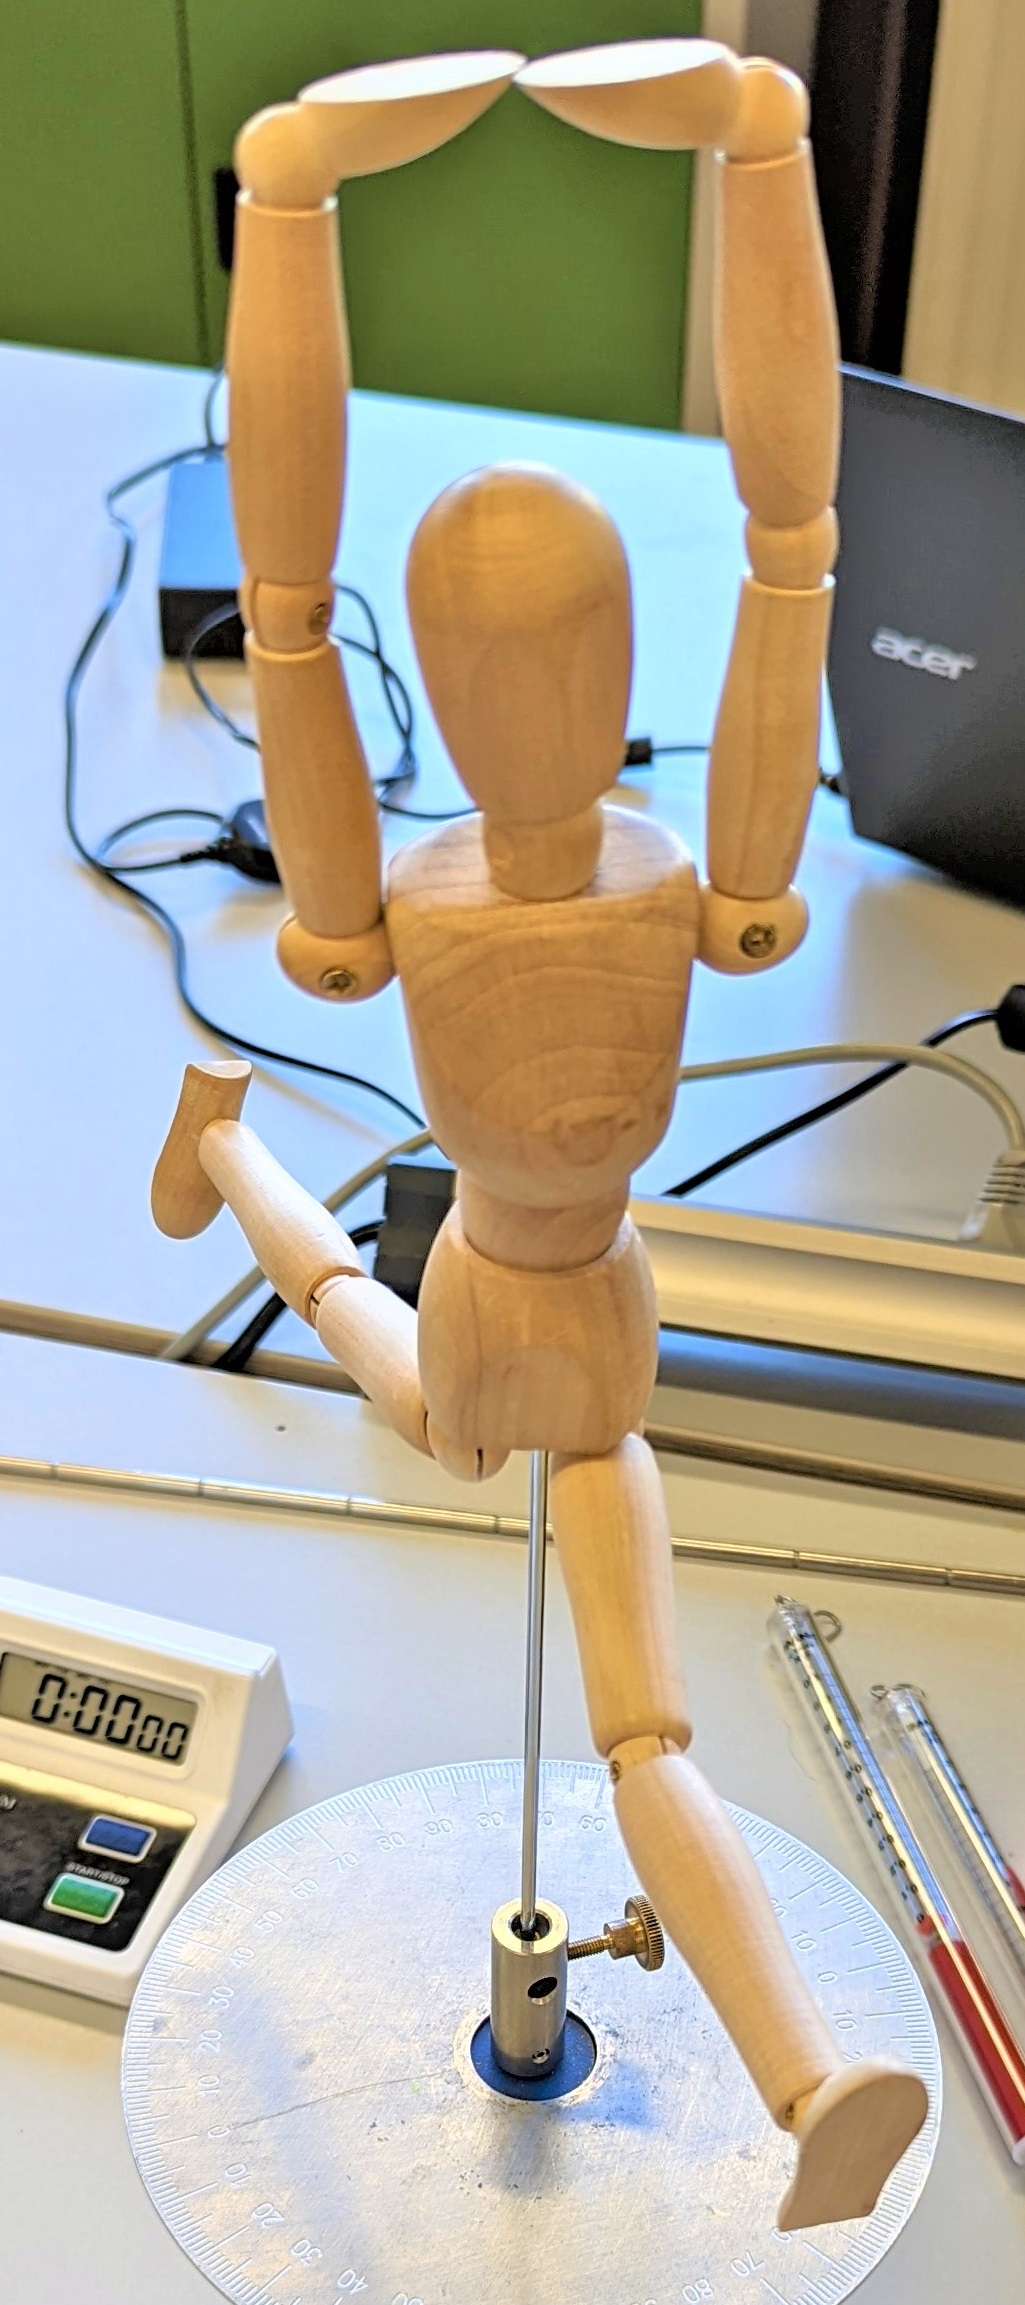
\includegraphics[width=0.6\textwidth]{content/Ballet3.jpg}
  \end{subfigure}
  \hfill
  \begin{subfigure}{0.48\textwidth}
      \centering
      \caption{Stellung 2}
      \label{fig:D_Holzpuppe2}
      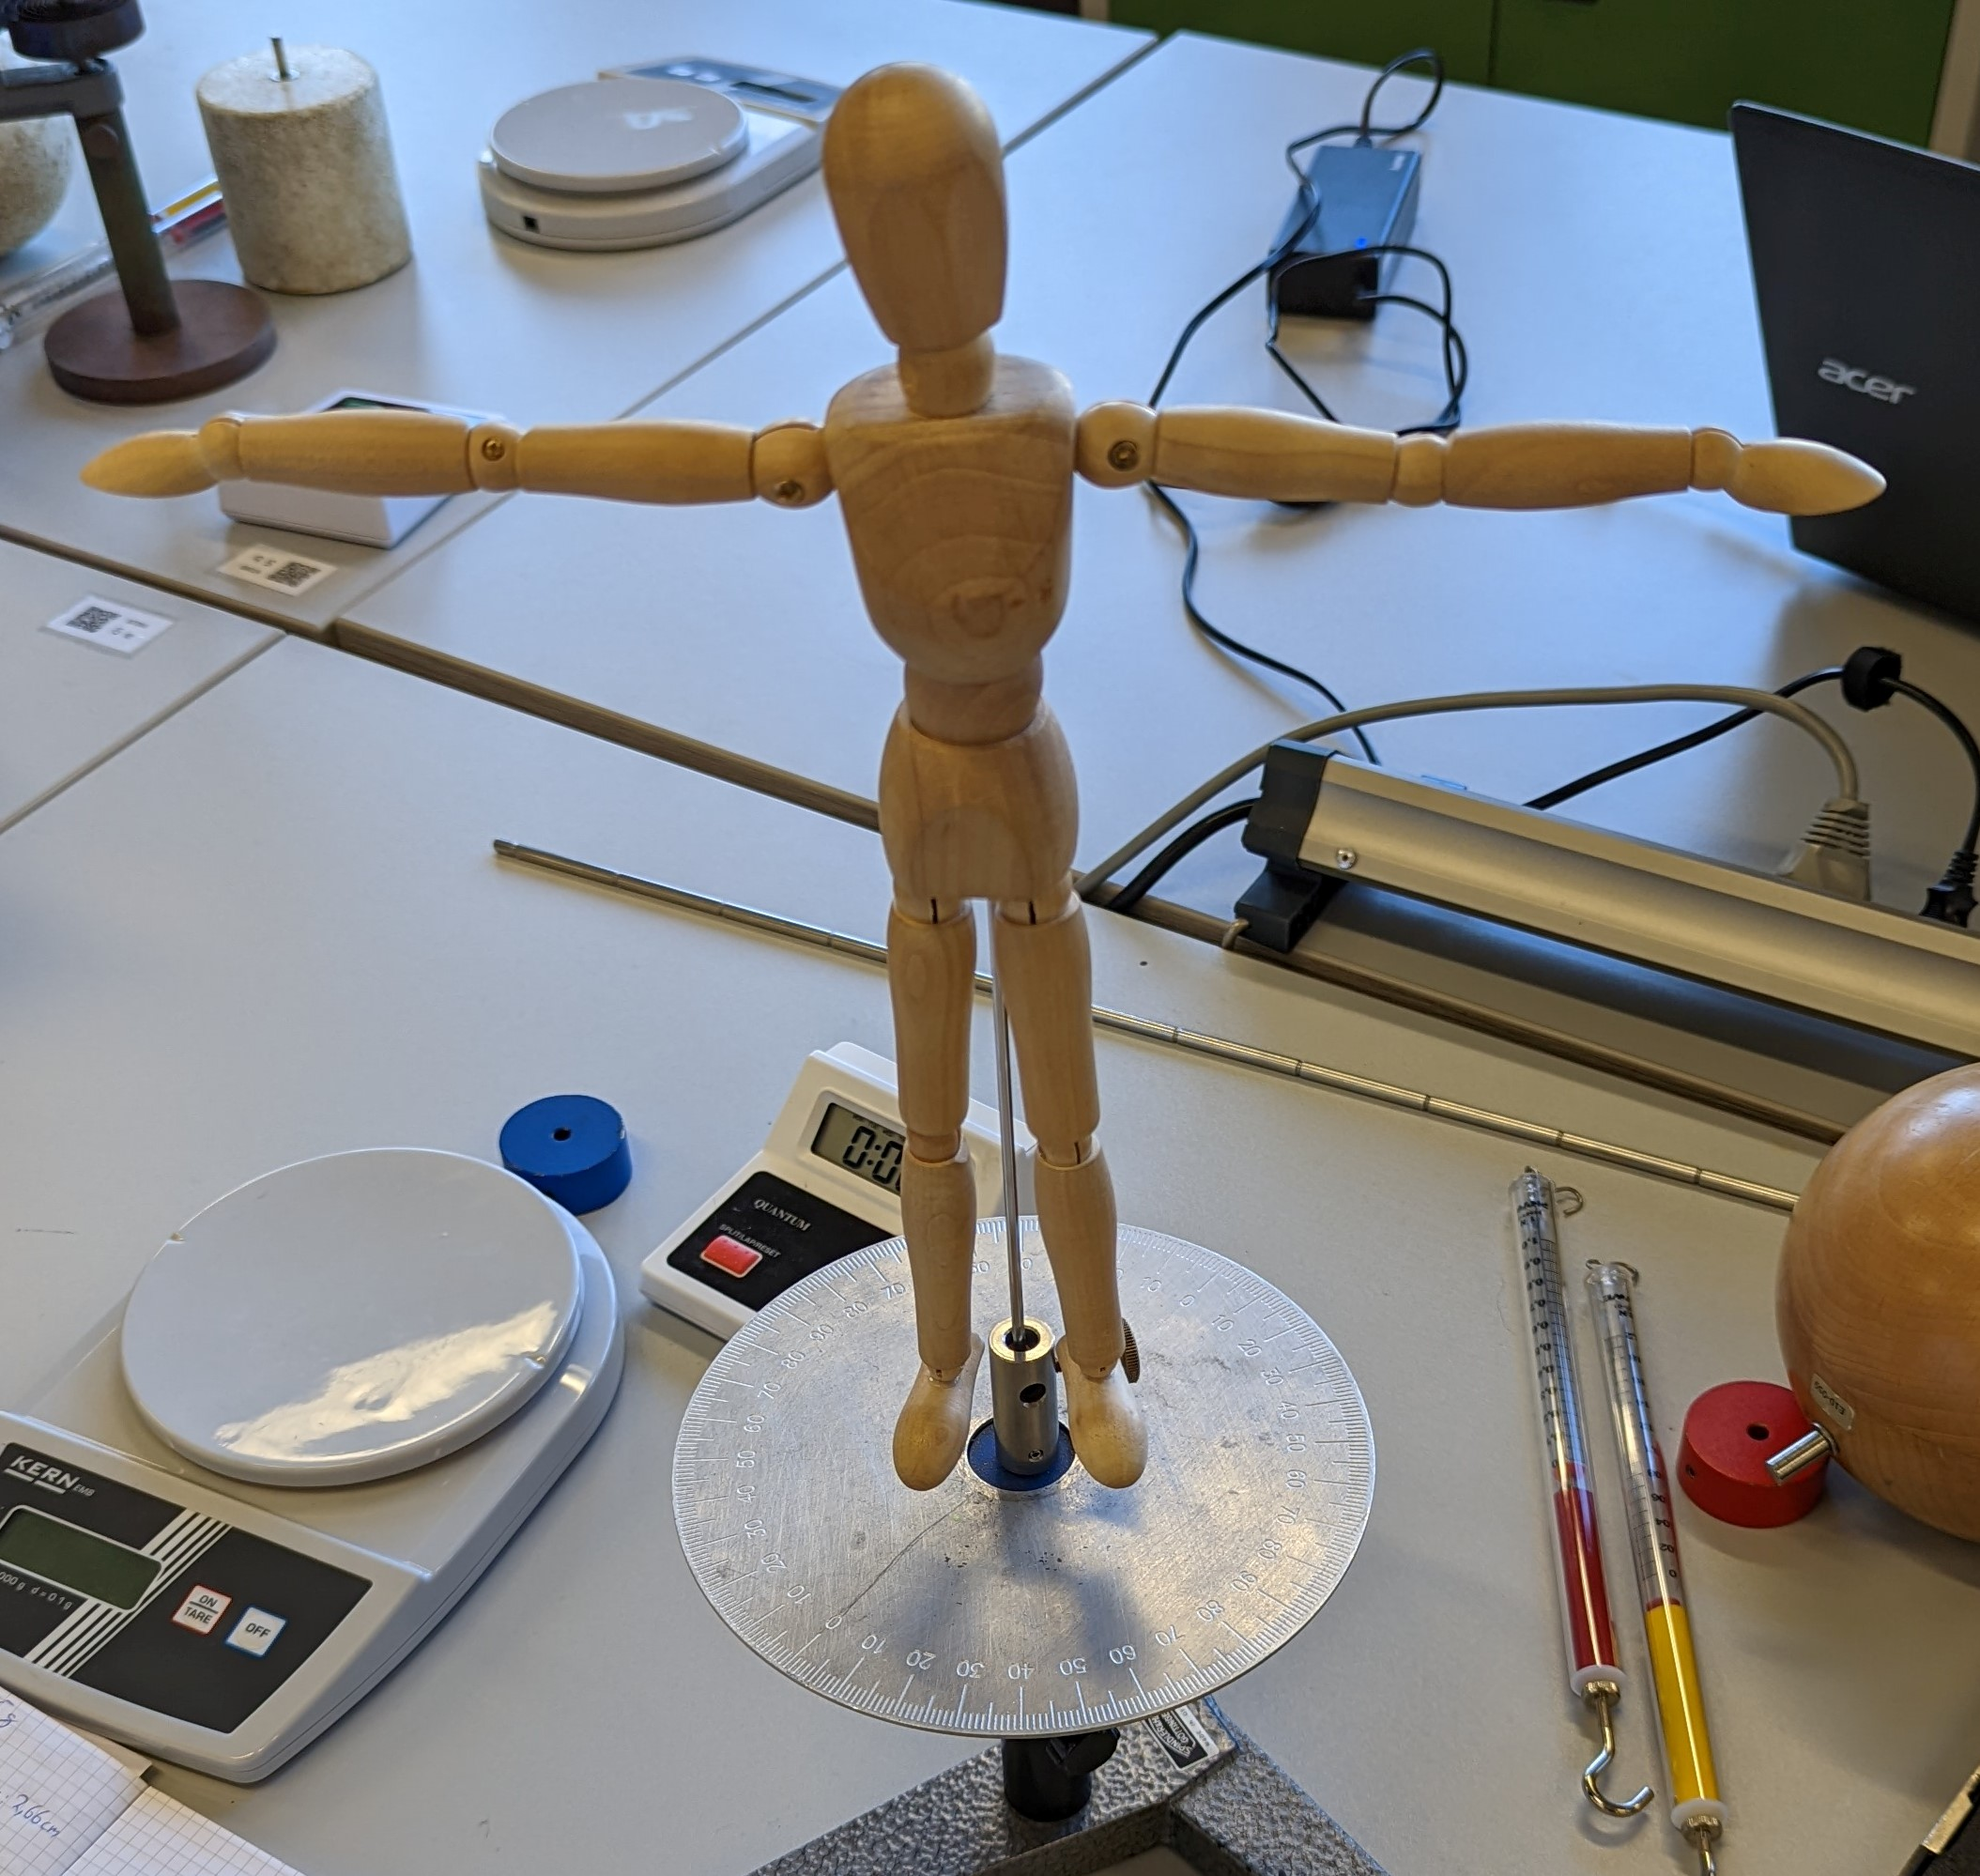
\includegraphics[width=0.8\textwidth]{content/T_Pose3.jpg}
  \end{subfigure}    
\end{figure}

\subsubsection{Trägheitsmoment der ersten Stellung}
\label{subsubsec:A_ballet}
Die Stellung der Figur ist in \autoref{fig:D_Holzpuppe1} dargestellt. Zunächst werden die gemessenen Schwingungsdauern, welche dem Anhang entnommen werden können, der Figur in Stellung 1 gemittlet.
Dieser lautet $\overline{T}_1 = \qty{0.751+-0.028}{\second}$. 
Dann wird mit \autoref{eqn:I_K} das experimentelle Trägheitsmoment bestimmt. Dadurch ergibt sich $I_{1,\text{exp}} = \qty{0.684+-0.180}{\gram\metre\squared}$. Der Theoriewert eine komplexen
Körpers muss mit dem Satz von Steiner berechnet werden. Dazu werden zunächst die theoretischen Trägheitsmomente der einzelnen Körperteile berechnet, welche dann abschließend addiert werden.
Die Einzelträgheitsmomente können \autoref{tab:einzelträgheitsmomente} entnommen werden.
\begin{table}
  \centering
  \caption{Einzelträgheitsmomente der Holzpuppe.} 
  \label{tab:einzelträgheitsmomente}
  \begin{tabular}{l c @{${}\pm{}$} l c @{${}\pm{}$} l}
      \toprule
      & \multicolumn{2}{c}{Stellung 1} & \multicolumn{2}{c}{Stellung 2} \\
      \cmidrule(lr){2-3}\cmidrule(lr){4-5}
       & \multicolumn{2}{c}{$\unit{I_{1,\text{theo}}\per\micro\gram\metre\squared}$} & \multicolumn{2}{c}{$\unit{I_{2,\text{theo}}\per\micro\gram\metre\squared}$} \\
      \midrule
      {Kopf} & 1.6 & 0.6 & 1.6 & 0.6 \\
      {Arme} & 8.9 & 1.9 & 113 & 19 \\
      {Rumpf} & 14 & 4 & 14 & 4 \\
      {Beine} & 106 & 22 & 2.8 & 0.6 \\
      \bottomrule 
  \end{tabular}
\end{table}
Nun werden alle Einzelträgheitsmomente der Stellung 1 addiert. Das theoretische Gesamtträgheitsmoment in der Stellung 1 beträgt dann $I_{1,\text{Ges},\text{theo}} = \qty{0.246+-0.040}{\gram\metre\squared}$.
\subsubsection{Trägheitsmoment der zweiten Stellung}
\label{subsubsec:A_tpose}
Wie zuvor wird ebenfalls als erstes der Mittelwert der Periodendauer in Stellung 2 gebildet. Dieser beträgt $\overline{T}_2 = \qty{0.637+-0.012}{\second}$. Mit diesem Wert kann erneut mittels \autoref{eqn:I_K}
das experimentelle Trägheitsmoment errechnet werden. Daher ergibt sich $I_{2,\text{exp}} = \qty{0.493+-0.125}{\gram\metre\squared}$. Für den Theoriewert werden nun die Einzelträgheitsmomente addiert, 
welche \autoref{tab:einzelträgheitsmomente} entnommen werden können. Der Theoriewert zu zweiten Stellung lautet dann $I_{2,\text{theo}} = \qty{0.247+-0.037}{\gram\metre\squared}$.
